\documentclass{llncs}  % from http://www.springer.de/comp/lncs/authors.html
\usepackage[dvips]{graphicx}
\usepackage{oz}

% Temporary, until I get the Zstan package.
\newcommand{\AFont}[1]{\texttt{#1}}
\newcommand{\CADiZ}{CADiZ}
\newcommand{\Zeta}{Zeta}
\newcommand{\ASpecification}{Specification}
\newcommand{\ASection}{Section}
\newcommand{\AParagraph}{Paragraph}
\newcommand{\APredicate}{Predicate}
\newcommand{\AExpression}{Expression}
\newcommand{\TNAME}{TNAME}
\newcommand{\ASectTypeEnv}{SectTypeEnv}
\newcommand{\ASignature}{Signature}
\newcommand{\CFreetype}{Freetype}
\newcommand{\CBranch}{Branch}
\newcommand{\CPrec}{Prec}
\newcommand{\CAssoc}{Assoc}
\newcommand{\DTanonspec}{\par TODO: show DTanonspec here \par}
\newcommand{\DTschemadef}{\par TODO: show DTschemadef here \par}
\newcommand{\DTgenschemadef}{\par TODO: show DTgenschemadef here \par}
\newcommand{\DThorizdef}{\par TODO: show DThorizdef here \par}
\newcommand{\DTgenhorizdef}{\par TODO: show DTgenhorizdef here \par}

\newcommand{\TODO}[1]{\textbf{TODO: #1}}   % For draft version
% \newcommand{\TODO}[1]{}    % For final version

\title{ZML: XML Support for Standard Z}
\author{Mark Utting\inst{1} 
        \and Ian Toyn\inst{2}
        \and Jing SUN\inst{4}
        \and Andrew Martin\inst{3}   % and perhaps David Curry?
        \and Jin Song DONG\inst{4}
        \and Nicholas Daley\inst{1}
}
\institute{The University of Waikato, Hamilton, NZ\\
        Email: \texttt{\{marku,ntd1\}@cs.waikato.ac.nz}
  \and  The University of York\\
        Email: \texttt{ian@cs.york.ac.uk}
  \and  Oxford University\\
        Email: \texttt{Andrew.Martin@comlab.ox.ac.uk}
  \and  The National University of Singapore \\
        Email: \texttt{\{sunjing,dongjs\}@comp.nus.edu.sg}
}

\begin{document}
\maketitle

\begin{abstract}
  This paper proposes an XML format for standard Z.
  We describe several earlier XML proposals for Z,
  the problems and issues that arose, and the rationales
  behind our new proposal.
  The new proposal is based upon a comparison of various existing Z
  annotated syntaxes, to ensure that the mark-up will be widely usable.
  This XML format is expected to become a central feature of
  the CZT (Community Z Tools) initiative.
\end{abstract}

\section{Why an XML format for Z?}

The publication during 2002 of the ISO Z Standard~\cite{ISO13568}
represents a significant milestone for the development and
interoperability of Z tools.  However, technology has advanced during the
development of the standard, so it now seems most natural for tools
to interact using an XML mark-up \cite{xml-standard}.

This paper describes such a mark-up, intended to be a development of the
Standard's work, as a contribution to the Community Z Tools (CZT)
initiative.  CZT has been proposed in response to the observation that
many interesting Z tools have been developed, but few have built large
user communities, and many have found it necessary to invest
disproportionately large amounts of effort in the relatively mundane
activities of parser and pretty-printer development.  The initiative aims
to define interfaces and interchange facilities (and later, code
libraries) which Z tool developers can draw on in an open-source spirit,
with the aim both of promoting interoperability and of relieving those
wishing to develop novel tools for visualisation, animation, refinement,
proof, and so on, from the need to invest effort in the user interface
code.

XML is a development, like HTML, from the SGML.  Early drafts of the Z
Standard included an SGML mark-up, but it was found hard to maintain. XML
now enjoys a much wider take-up than SGML, having quickly become a new
standard for structured information interchage between tools (`the ASCII
of the new century').

Without such a mark-up, Standard Z allows specifications to be exchanged
using Unicode (UCS\cite{ISO10646-1,ISO10646-2}).
However, this representation is suitable only
for interchanging raw (unparsed) Z specifications, without annotation.
Tools (and sometimes authors) benefit from being able to annotate terms
with type information, anticipated usage and refinement targets, free-form
comments, and so on.   A particular presentation (on paper, on screen, or
within program data structures) may make use of some of these annotations
and discard others.  An XML format facilitates the inclusion of such
annotations, with as little or as much structure as is appropriate.  In
the longer term, when this use of XML reaches greater maturity, we would
expect the format described here to become part of the ISO Z Standard.


\subsection{Requirements of a Z interchange mark-up}\label{injectivity}

We have four requirements for an XML mark-up for Z:
 
\paragraph{Annotations}
The already mentioned annotations should be accommodated
in the interchange mark-up wherever tools wish to put them.
The forms of individual annotations should not be constrained.
There should be some standard annotations for types and for
source-file locations (so that error messages can refer to the
source of an error), but it should also be possible for tools
to define additional annotations.  Tools that do not understand
such annotations should simply ignore them.

\paragraph{Injectivity}
The concrete syntax of Z provides different ways of specifying the 
same things.  For example, a boxed schema paragraph
may be written in an equivalent definitional form, without the box.
After a specification has been transferred between tools, the user wants
to be reassured as much as possible (by avoiding unexpected changes 
of presentation) that their specification document has not been changed.
Consequently, the interchange mark-up for Z should capture
sufficient information from the concrete representation 
to be able to resurrect the same concrete phrases
(though not necessarily the same layout).
In other words, we want the conversion of a textual Z specification into 
XML format to be one-to-one (injective), so that the concrete 
representation before and after interchange, ignoring annotations,
remains recognisably the same.
For the schema paragraph example, this means keeping a note of whether 
or not the boxed representation is used. 
In this paper, we avoid using the traditional term \textit{abstract syntax}
because of this avoidance of loss of information from the concrete form.

\paragraph{Commonality}
Conversely, for reasons of simplicity and demonstrable soundness, 
tools should need to deal with as few cases as possible.  This implies
that we should merge equivalent concrete constructs whenever possible
(the Z standard has a large number of transformation rules that do
exactly this).
For example, a tool might offer to display the section-type environment
of a schema paragraph regardless of whether or not it is boxed.
This is easier if a common \textit{annotated syntax} is used
for both of the concrete representations of the schema paragraph.
Interchange will be eased if the mark-up is based on an annotated syntax
that identifies similar commonalities to those exploited by tools.

In this paper, we merge many constructs, but preserve injectivity
by adding attributes that identify which of the concrete syntax formats
was used.  In other places, we use distinct XML tags for similar
constructs, but define these tags using type hierarchies that reflect 
the commonalities. 

\paragraph{Correspondance with Java Class Hierarchy}
As well as defining an interchange format, one of the CZT 
aims is to develop a Java library for building Z tools.  
This means we want Java data structures for Z, plus various
common operations on those data structures, such as type checking,
and transformation tools.  This will make it easier to develop new
Z tools, and to fit them into a common framework.
We want to develop Java class hierarchies
that closely match the structure of the XML format.  
This paper shows that by using XML schema to define the XML format,
we can get a natural mapping between the XML schema definitions and
an elegant object-oriented hierarchy of Java classes.

\vspace{1.5ex}

The annotated syntaxes used within existing tools have already
addressed these issues of annotations, commonalities and injectivity.
The annotated syntax used within Standard Z addresses some of these issues.
An interchange mark-up for Z will be easier for a tool to use
if the mark-up is similar to the tool's own annotated syntax,
but there is considerable variation between the syntax used within existing
tools. 

This document compares some existing annotated syntaxes
and describes an XML mark-up that will be usable by the compared tools.
An interchange mark-up for Z will be successful only if
it can be used by many Z tools, so we are interested to 
receive feedback from other tool builders.


\subsection{DTD or XML Schema?}

The syntax of XML\cite{XML} is trivial,
making it easy for tools to generate and parse,
but its syntactic monotony provides little help to a human reader
trying to comprehend the content of an XML document.
XML mark-up is not something that the sane would want to write by hand.
Expectations on the content of an XML document---how values are
structured---can be specified separately (by hand by Z experts),
then conformance to the specification can be checked automatically
(by a \textit{validating parser}).
Such a specification can be written in either of two languages:
as a \textit{Document Type Definition} (DTD), or as an \textit{XML Schema}.
The simple syntax of XML allows tools to communicate
without a DTD or XML Schema (using a \textit{non-validating parser}),
but such a specification is nevertheless useful to toolbuilders
in defining what the tools should be able to interchange.

The DTD notation is older and simpler than the XML schema notation,
and more human-readable.  It also allows specification of names for
entities, which the XML schema language does not---entities are
desirable for Z, since they would allow each toolkit operator to be
given a meaningful name rather than specifying the raw unicode characters.

The XML Schema language allows better specification of the data types
of elements than the DTD language. In addition to the built-in
datatypes such as string, integer, boolean, float, data time and so
on, XML Schema provides mechanisms to further constrain the allowable
content of an element or attribute, such as setting a valid range of
values or defining a regular expression to which the content must
conform. Furthermore, XML schemas are themselves written in XML.  This
makes the document descriptions more verbose, but also far more
extensible than they were in the original DTD syntax. Declarations can
have richer and more complex internal structures than declarations in
DTDs. Thus XML Schemas can be stored along with other XML documents in
XML-oriented data stores, referenced, and even styled, using tools
like XLink, XPointer, and XSL. For our purposes, we prefer to use XML
schema notation, to obtain a tighter specification of the structure,
and to take advantage of XML tools, such as XSLT.


\section{Previous Work}

There were earlier attempts to define XML mark-ups for Z
\cite{Dong01,Wordsworth99,ZEVES???}, but these did not support the
interchange of annotations such as the types of expressions, and were
based on an earlier version of Z~\cite{spivey:z-notation2}.

Before ZB2002, Ian Toyn wrote a DTD for Z, based on the abstract
syntax of the Z standard, plus ideas from CadiZ and Zeta.  This
DTD has heavily influenced our proposal in this paper.

For example, here is the top-level element declaration from that DTD:
\begin{small}
\begin{verbatim}
<!ELEMENT Z:Spec; (((Z:Sect;*), Z:SpecAnns;?) | Z:PCDATA)>
\end{verbatim}
\end{small}

This defines a Z specification to be either a sequence of sections
followed by an optional \emph{specification annotation}, or a
\AFont{PCDATA} alternative, which is another element that is defined 
to contain just \verb!#PCDATA! (\textit{parsed character data}).
Every element in the DTD includes a \AFont{Z:PCDATA} alternative, so
that if one part of a specification contains an error, the whole
specification can still be passed between tools.  For example,
a fully-parsed specification might be passed to an editor, and after
editing is complete, the editor might pass it back with unchanged
portions still in parsed form, but the edited portions in \AFont{Z:PCDATA}
form. 

During 2002, David Currie validated the DTD, and Utting and Daley
derived a Java class hierarchy from it~\cite{daley:report02}.
During this process, we identified several difficulties with the
DTD structure:

\begin{enumerate}
\item The presence of an `unparsed' alternative for \emph{every} element
  allowed extremely fine-grained portions of the specification to be left
  unparsed, but dramatically complicated the Java class hierarchy.
  Basically, every element \verb!E! of the DTD had to be translated into
  \emph{three} Java classes: an abstract class \verb!E! and two concrete 
  subclasses, \verb!EParsed! and \verb!EUnparsed!, where \verb!EParsed!
  contained fields that matched the parsed structure and \verb!EUnparsed!
  contained just an unparsed string.  The real disadvantage of this was
  that every piece of Java code that accessed an \verb!E! object had to
  immediately check whether it was parsed or unparsed.  This issue was not
  specific to Java, but would affect processing in every language.
  
  To solve this problem, our new proposal in this paper limits the
  \emph{granularity} of the unparsed portions so that an entire paragraph
  (for example, one schema or one equality definition) is the smallest
  unparsed portion allowable.  This simplifies processing, because it means
  that only the top-level of processing needs to consider unparsed portions
  and once we see a parsed paragraph, we know that everything inside it
  will also be parsed.

\item The combination of `unparsed' alternatives and attributes
  gives some strange effects.  For example, binary predicates are
  defined as usually having two children, plus a compulsory attribute
  that indicates which logical operator is used to combine them.
\begin{small}
\begin{verbatim}
<!ELEMENT Z:LogPred; ((Z:Pred;, Z:Pred;, Z:LogPredAnns;?) | Z:PCDATA)>
<!ATTLIST Z:LogPred; Z:Log; (And|Or|Imp|Iff|Nl|Semi|Chain) #REQUIRED>
\end{verbatim}
\end{small}
  This means that the logical operator must be specified,
  even for the unparsed alternative, which is not sensible. 

  This problem disappears when paragraphs are the smallest unparsed unit.

\item Each element in the DTD has its own kind of annotation, as
  illustrated in the examples above.  Each kind of annotation is given
  a default definition in the DTD (expression annotations contain just a
  type, schema annotations contain a signature etc.), but can be
  overridden by providing an extended DTD that adds extra fields.
  However, because each kind of expression has its own kind of annotation,
  it is necessary to override all 23 kinds of expression annotations
  to add a new annotation to expressions (or 7 kinds for predicates, 
  5 kinds for paragraphs, etc.).
  
  To solve this problem, and make it easier to add new kinds of
  annotations, we have changed to a more loosely-typed view of annotations
  that is similar to the annotations in Zeta.  Each Z construct can contain
  a list of arbitrary annotations.  Each annotation has a \verb!Kind!
  field, which is a token that indicates the type of the annotation.  This
  means that a tool could attach an annotation to an inappropriate
  construct (such as putting a type annotation on a predicate), but such
  annotations do no harm and can simply be ignored.  On the other hand,
  there are many kinds of annotations (such as hyperlinks, source-code
  positions and comments), that we want to be able to attach to arbitrary
  constructs, and this is easier with these loosely-typed annotations.
  
\item In an object-oriented class hierarchy, it is possible to organise
  the hierarchy to reflect commonality, so that common fields and methods
  can be inherited.  This is more flexible than the DTD structure, which
  does not have any kind of inheritance.  This resulted in more differences
  between the DTD structure and our ideal Java class hierarchy than we
  would have liked. 

  Our new proposal solves this problem by using XML schema to specify the
  structure of the Z markup.  XML schema offers a rich set of (single)
  inheritance features between types, as well as a \emph{substitution
  group} facility which is similar to subtyping in object-oriented
  languages.  
\end{enumerate}


Also in 2002, at the National University of Singapore, Dong and Sun
developed a new version of their XML schema, based more closely on
the annotated syntax structure of the Z standard.  This did not
support unparsed alternatives or annotations, and made less use of
commonalities than Toyn's DTD, but it included extensions 
for supporting Object-Z and TCOZ (Timed Communicating Object Z)~\cite{md99a}.
They demonstrated that it is possible to use the XSLT transformation
language to transform the XML form of Z into elegant HTML with proper boxes
and mathematical Unicode fonts\footnote{If you have an appropriate Unicode
  font on your computer, such as Microsoft Arial Unicode.  See
  \url{http://nt-appn.comp.nus.edu.sg/fm/zml/z-stand/zml-xsd.htm} for 
  a demonstration of this system.} 
The generated HTML includes hyperlink crossreferences, and buttons for
expanding schema expressions and folding them again.  The truly impressive
feature is that this transformation system actually runs in your own
browser, using standard technologies (XML, XSLT and Unicode).

This shows the promise of our XML proposal---one can download a parsed
and type-checked Z specification in an XML format that is ideal for
importing into tools, yet still view it and explore it (following
cross references etc.) with a standard web browser.

Furthermore, Dong and Sun have defined an XSLT stylesheet for
automatically transforming the Object-Z/TCOZ models in XML into UML
class diagrams~\cite{sun01www}. The XSLT encodes the projection rules
from the formal notations into their corresponding UML
counterparts. Recently this work has been extended to support the
auto-generation of UML statechart diagrams from Object-Z/TCOZ
specifications via Java XML parser~\cite{dong02icfem}. Both
implementations take the customized XML format as a standard input and
performs XML transformation into XMI (XML Metadata Interchange) format
for visualization. In addition, an XML-base typer checker was built
for the static type checking of Z/Object-Z/TCOZ specifications in XML
format.


\section{Influences on our Design}

The structure of our proposed XML markup is based on Ian Toyn's DTD,
which was designed by comparing and merging the best features
of three annotated syntaxes used by the Z standard and existing tools.
This section briefly describes each of these systems and how they
differ from our goals.

\subsection{Standard Z}

Standard Z's annotated syntax provides the basis for its definition
of the type system and semantics of Z.
These are the only functions defined on its annotated syntax.
In particular, the standard has no need to resurrect concrete syntax.
It has annotations for types of expressions,
signatures of paragraphs, and section-type environments of sections.
Commonalities are identified by \textit{syntactic transformation rules},
which define the translation of concrete syntax to equivalent annotated syntax.
Some of these syntactic transformation rules will be quoted below.

XML mark-up will differ from Standard Z's annotated syntax
because of the need to resurrect concrete syntax
and the need to support a greater variety of functions and annotations.

\subsection{\CADiZ}

\CADiZ's annotated syntax supports typechecking,
prettyprinting (i.e.\ resurrection of concrete syntax),
interactive browsing (i.e.\ tracking of references to declarations
and inspection of types, signatures and environments),
and logical inference (i.e.\ transformation to equivalent notation,
as in the course of proofs).
Z notation is also used as patterns in tactics for automated reasoning.

In \CADiZ's annotated syntax,
the representation of declarations plays many roles.
As well as representing the name and expression of a declaration,
it records the declared variable's type,
allowing signatures to be represented as lists of declarations,
and it records which expressions refer to it.
An inclusion declaration brings new copies of a declaration into scope,
so that uses of the included declaration are not
confused with uses of the original declaration.
Expressions record the declarations to which they refer.
These records support interactive browsing.
They also support logical inference rules
regardless of variable capture side-conditions:
the inference maintains bindings of references to declarations,
and the prettyprinter does renaming
wherever variable capture would otherwise appear to occur.
The representation of declarations causes \CADiZ's annotated syntax
to be not a tree structure but a more general graph,
which would be inconvenient for a textual interchange mark-up such as XML
(but more on this later).

\CADiZ\cite{CADiZ} can be said to support Standard Z---the deviations
are very minor.
(It does have some extensions to Standard Z, but we will ignore those.)
\CADiZ's annotated syntax is not fixed, and has changed frequently in the
past (and may change in the future to be closer to this proposal). 

\subsection{\Zeta}

\Zeta's annotated syntax supports typechecking,
prettyprinting (i.e.\ resurrection of concrete syntax),
and animation (i.e.\ automatic reduction of expressions).
(Those are the functions of the core edition of \Zeta.)

XML mark-up will differ from \Zeta's annotated syntax
wherever \Zeta\cite{Zeta} deviates from Standard Z.

\subsection{Standard Terminology}

The main syntactic rules (Specification, Section, Paragraph, Predicate and
Expression) are present in all annotated syntaxes for Z, though not with
the same names.  In some tools, this renaming reflects the widening of
syntactic rules to include non-Z phrases.  The following table summarises
these names, and suggests names to be used for the elements in XML.
(The \verb!Z:! prefix is just a namespace prefix, and can be omitted
in XML documents whose default namespace is our XML schema).

\begin{center}
\begin{tabular}{|l|l|l|l|}
\hline
{\bf Standard Z} & {\bf \CADiZ} & {\bf \Zeta} & {\bf XML}\\
\hline
\ASpecification & \AFont{[doc]} & \AFont{UnitAbsy[]} & \AFont{Z:Spec}\\
\ASection & \AFont{doc} & \AFont{UnitAbsy.Section} & \AFont{Z:Sect}\\
\AParagraph & \AFont{def} & \AFont{Item} & \AFont{Z:Para}\\
\APredicate & \AFont{pred} & \AFont{Predicate} & \AFont{Z:Pred}\\
\AExpression & \AFont{term} & \AFont{Expr} & \AFont{Z:Expr}\\
\hline
\end{tabular}
\end{center}


\section{Our XML Schema Proposal}

In this section, we go through each major construct of the
Z notation, briefly comparing the Z standard, \CADiZ\ and \Zeta,
and describing our proposed XML structure.  The XML schema was
developed and validated using the XML-Spy tool\footnote{See
  www.xmlspy.com}, and the diagrams were also generated by XML-Spy.

\subsection{Specifications and Sections}\label{Specification}

Standard Z specifications are either anonymous or sectioned.
The standard syntactically transforms anonymous specifications
to sectioned specifications, as follows (Z standard, clause 12.2.1.1).
\DTanonspec
The name $Specification$ can be anything distinct.
Concrete syntax may be resurrected by recognising the distinct name.
\TODO{Let us propose a specific name.  Say `anonymous'?  Or
  `Specification'?}

So, a specification can be represented as just a sequence of sections,
and both \CADiZ\ and \Zeta\ use that representation.
The following table lists the components of a Z section.
\begin{center}
\begin{tabular}{|l|l|l|l|}
\hline
{\bf Standard Z} & {\bf \CADiZ} & {\bf \Zeta} & {\bf XML}\\
\ASection & \AFont{doc} & \AFont{UnitAbsy.Section} & \AFont{Z:Sect}\\
\hline
\TNAME & \AFont{word} & \AFont{Name} & \AFont{Z:Word}\\
\AFont{seq} \TNAME & \AFont{[parent]} & \AFont{Name[]} & \AFont{Z:Word*}\\
\AFont{seq} \AParagraph & \AFont{[def]} & \AFont{Item[]} & \AFont{Z:Para*}\\
\ASectTypeEnv & & & \AFont{Z:SectAnns?}\\
\hline
\end{tabular}
\end{center}

Fig.~\ref{fig:spec}
shows the corresponding XML structure: a specification is a sequence of
zero or more sections, where each section has a name, some parents, 
some paragraphs and possibly some annotations.  In addition, the
\AFont{Spec} element has three optional attributes to record its
\emph{Creator} and the \emph{Date} and \emph{Time} of the last
modification. 
\TODO{Allow annotations on the whole specification?}

Within a \AFont{Sect}, the list of parent names need not include
\textit{prelude}, as that is implicitly a parent of all sections.
If there are no parents,
the \AFont{Sect} element does not record whether or not
the keyword \AFont{parents} occurred in the concrete representation.
This doesn't matter sufficiently to deserve the declaration of an attribute.

\begin{figure}[htbp]
  \centering
  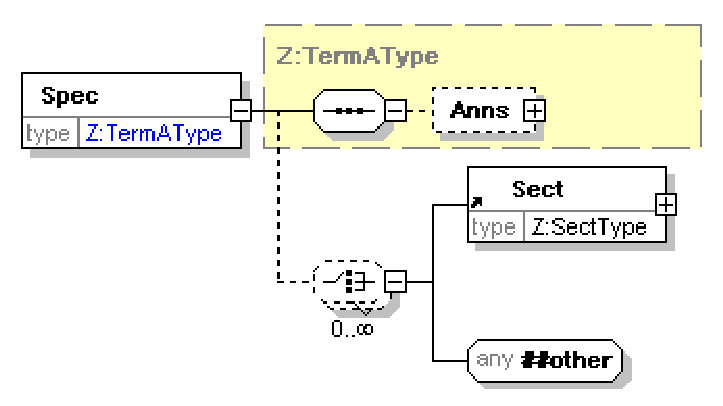
\includegraphics[width=\textwidth]{spec.eps}
  \caption{XML structure for an entire Specification}
  \label{fig:spec}
\end{figure}

\TODO{Include Ian's complete small XML example here, in which
  the whole spec is unparsed?  Oh dear!  My XML structure does not
  allow that!  :-)  Perhaps we could put the whole specification into
  one paragraph?   :-)}

Another important feature that is not shown in Fig.~\ref{fig:spec} is that
both \AFont{Spec} and \AFont{Sect} have the XML \AFont{mixed} flag set to
\AFont{true} (it is \AFont{false} for all other constructs).  This means
that arbitrary text is allowed to be interspersed between sections and
between paragraphs, which supports the usual Z style of interleaving formal
specification and explanation.

\TODO{It might be nice here to allow arbitrary TAGS within sections too, so
  that the Z tools just skip over other XML content that is not Z-related?
  Is there a way of saying that any other tags are allowed,
  provided they belong to a different namespace?}

\TODO{ Another design issue is, what should a standard Z tool do when it
  sees a Z extension paragraph?  Quietly ignore it or treat this as an
  error?  } 


\subsection{Paragraphs}

Ian Toyn's DTD defined \verb!Z:Para! to be a \emph{choice} between six
kinds of paragraph.  XML Schema gives us several different ways of doing
this, and we have decided to use a newish XML Schema feature,
\emph{Substitution Groups}, rather than choice groups, because substitution
groups are similar to an object-oriented subtyping structure (where a
subtype object can replace a supertype object), and can support inheritance
of attributes and elements.   

Substitution groups make it easy to extend the structure.  For example, a Z
extension could add a new kind of paragraph simply by defining a new
element with \texttt{substitutionGroup="Para"}.  It is also easy to add new
features to one of the subtypes, like \texttt{AxPara}, by declaring a new
element whose type extends or restricts the type of \texttt{AxPara} and
says \texttt{substitutionGroup="AxPara"} (the substitution relationship is
transitive).

For example, here is the XML Schema definitions of paragraph and one of its
`subclasses', axiomatic paragraph.  We declare the \texttt{Para} element to
be abstract, so that XML files \emph{must} contain a specific kind of
paragraph, such as \texttt{AxPara} wherever a \texttt{Para} element is
expected.
\begin{verbatim}
<xs:element name="Para" abstract="true"/>
<xs:element name="AxPara" substitutionGroup="Para">
  <xs:complexType>
    <xs:sequence>
      <xs:element name="DeclName" type="DeclNameType" 
                  minOccurs="0" maxOccurs="unbounded"/>
      <xs:element name="SchText" type="SchTextType"/>
    </xs:sequence>
  </xs:complexType>
</xs:element>
\end{verbatim}

The following subsections go
through each kind of paragraph, describing their structure.


\subsubsection{Given Type Paragraphs}\label{giventypes}

The following table lists the components of a given types paragraph.

\begin{center}
\begin{tabular}{|l|l|l|l|}
\hline
{\bf Standard Z} & {\bf \CADiZ} & {\bf \Zeta} & {\bf XML}\\
Given types \AParagraph & \AFont{givdef} & \AFont{Item.AxiomaticDef[]} & \AFont{Z:GivenPara}\\
\hline
\AFont{seq} \TNAME & \AFont{[dec]} & \AFont{Expr.GivenType} & \AFont{Z:DeclName*}\\
\ASignature & & & \AFont{Z:GivenParaAnns?}\\
\hline
\end{tabular}
\end{center}

In \CADiZ, all declarations
(given types, generic parameters, variables)
share the same \AFont{dec} representation.
This has the advantage of providing a basis for
tracking all references to each declaration.
For the moment, I'm not worrying about
how to represent that information as annotations.

In \Zeta\ a given types paragraph is represented as
an \AFont{Item.AxiomaticDef}s sequence,
in which each \AFont{Item.AxiomaticDef}'s expression
is an \AFont{Expr.GivenType} containing the name of a given type.
This is an instance of a more general approach:
\Zeta\ represents each Z global definition as an \AFont{Item.AxiomaticDef},
using additional kinds of expressions beyond those of Standard Z
to make this possible.
We cannot see any additional advantages of this representation.
Concretely, a given types paragraph (or a single given type) is not an
expression, and so \Zeta's representation seems a bit forced. 

In XML, a given types paragraph is marked-up using
the \AFont{Z:GivenPara} element, as shown in Fig.~\ref{fig:givenpara}.
Note how annotations can be attached to the whole paragraph,
or to individual names (of given types) within the paragraph.
The same approach is followed throughout our XML structure---we allow
annotations to be attached to almost all constructs.  To save space in this
paper, we elide these optional annotations from the remaining diagrams.

\begin{figure}[htbp]
  \centering
  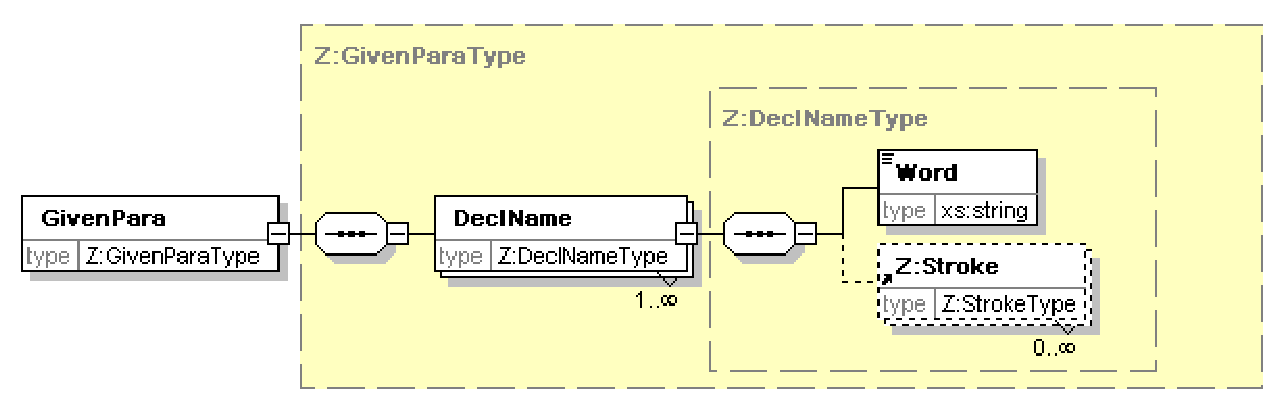
\includegraphics[width=\textwidth]{givenpara.eps}
  \caption{XML structure for Given Type paragraphs}
  \label{fig:givenpara}
\end{figure}


\subsubsection{Axiomatic Description Paragraphs}

The following table lists the components of an axiomatic description paragraph.

\begin{center}
\begin{tabular}{|l|l|l|l|}
\hline
{\bf Standard Z} & {\bf \CADiZ} & {\bf \Zeta} & {\bf XML}\\
(Generic) axiomatic description \AParagraph & \AFont{axidef} & \AFont{Item.AxiomaticDef} & \AFont{Z:AxPara}\\
\hline
\AFont{seq} \TNAME & \AFont{[dec]} & \AFont{NameDecl[]} & \AFont{Z:DeclName*}\\
\AExpression & \AFont{sch} & \AFont{Expr.Text} & \AFont{Z:Sch}\\
\ASignature & & & \AFont{Z:AxParaAnns?}\\
\hline
\end{tabular}
\end{center}

In \CADiZ\ and \Zeta,
non-generic axiomatic description paragraphs are represented
as generic ones with an empty list of generic parameters.
Standard Z differs, as it was thought that the semantics of generics
would be easier to understand if the semantics of non-generics
were defined separately first.

The declarations and predicate parts of an axiomatic description paragraph
are represented differently in the different annotated syntaxes.
Standard Z transforms them to an expression.
\CADiZ\ retains the schema text,
represented by a distinct rule in the annotated syntax.
\Zeta\ views the schema text as an expression.
We believe that some annotations can usefully be placed on schema texts,
and that any single expression appearing where a schema text is expected
is best represented as an inclusion in a schema text,
so that there is somewhere to record those annotations.

Fig.~\ref{fig:axpara} shows our XML structure for the \AFont{AxPara}
element, as well as for schema text and declarations.  Note the
three `subtypes' of \AFont{Decl}.  These are all declared as belonging to
the \AFont{Decl} substitution group so that they can appear wherever
a \AFont{Decl} is required.

The following definitions from the Z standard
(syntactic transformations 12.2.3.1---12.2.3.4)
show how to represent (generic) schema definition paragraphs
and (generic) horizontal definition paragraphs
as (generic) axiomatic description paragraphs.
\DTschemadef
\DTgenschemadef
\DThorizdef
\DTgenhorizdef
Generic operator definition paragraphs have their operator names
syntactically transformed to ordinary names
(syntactic transformations 12.2.9.1---12.2.9.4)
and hence they become generic horizontal definition paragraphs
that can be represented as generic axiomatic description paragraphs.

To support resurrection of the original concrete representation we add an
attribute \AFont{Box} with values: \AFont{OmitBox}, \AFont{AxBox} (the
default), or \AFont{SchBox}.  A further boolean attribute called
\AFont{Mixfix}, distinguishes whether mixfix syntax is used in the 
definition of a generic operator
e.g. $\_ \rel \_ [X,Y] == \power(X \cross Y)$.

\begin{figure}[htbp]
  \centering
  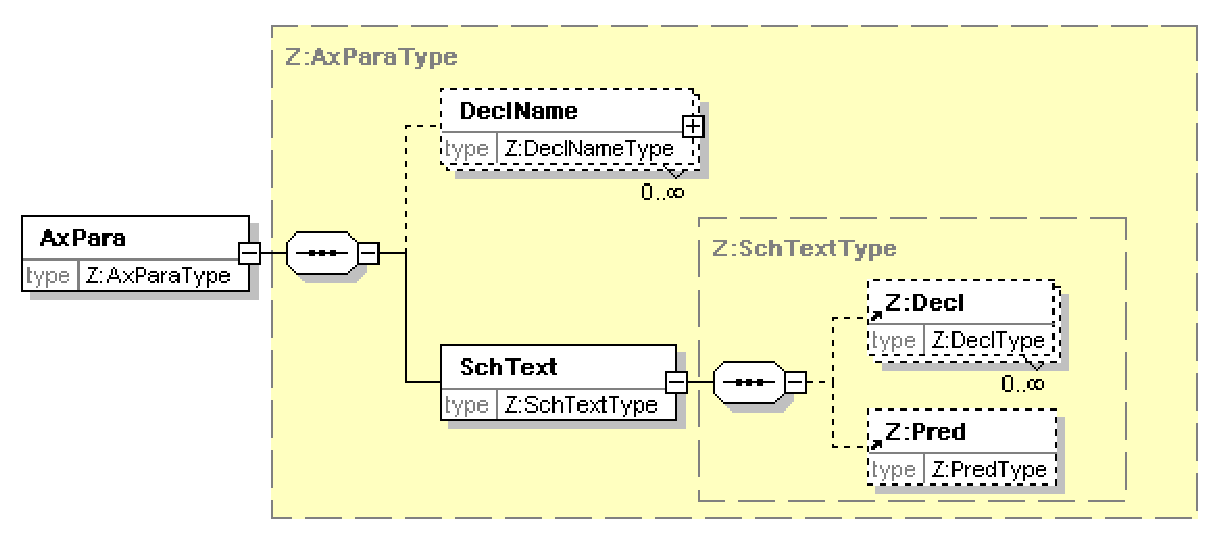
\includegraphics[width=\textwidth]{axpara.eps}
  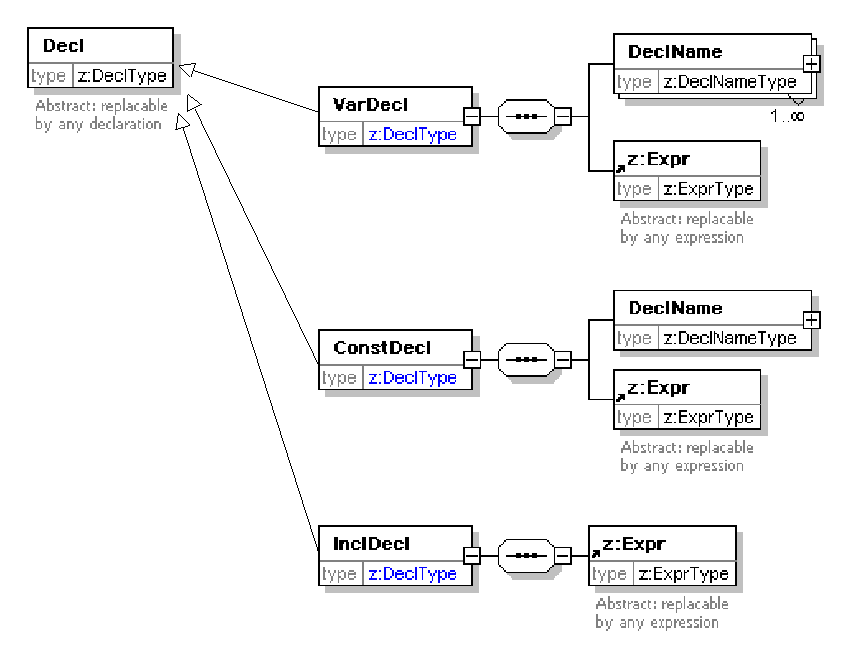
\includegraphics[width=0.8\textwidth]{decls.eps}
  \caption{XML structure for Axiomatic Definition paragraphs, Schema Text
  and Declarations}
  \label{fig:axpara}
\end{figure}

% \begin{figure}[htbp]
%   \centering
%   \caption{XML structure for declarations}
%   \label{fig:decls}
% \end{figure}


\subsubsection{Free Type Paragraphs}

The following tables list the components of a free types paragraph.

\begin{center}
\begin{tabular}{|l|l|l|l|}
\hline
{\bf Standard Z} & {\bf \CADiZ} & {\bf \Zeta} & {\bf XML}\\
Free types \AParagraph & \AFont{datdef} & \AFont{Item.AxiomaticDef[]} & \AFont{Z:FreePara}\\
\hline
\AFont{seq} \CFreetype & \AFont{[fret]} & \AFont{Expr.FreeType} & \AFont{Z:FreeType+}\\
\ASignature & & & \AFont{Z:FreeParaAnns?}\\
\hline
\end{tabular}
\end{center}

In \Zeta, the representation of free types paragraphs is similar to that of
other global definitions (see the earlier discussion in the Given Types
section).

\begin{center}
\begin{tabular}{|l|l|l|l|}
\hline
{\bf Standard Z} & {\bf \CADiZ} & {\bf \Zeta} & {\bf XML}\\
\CFreetype & \AFont{fret} & \AFont{Expr.FreeType} & \AFont{Z:FreeType}\\
\hline
\TNAME & \AFont{dec} & \AFont{NameDecl} & \AFont{Z:DeclName}\\
\AFont{seq} \CBranch & \AFont{[bra]} & \AFont{Branch[]} & \AFont{Z:Branch+}\\
 & & & \AFont{Z:FreeTypeAnns?}\\
\hline
\end{tabular}
\end{center}

The representation of a branch is very different in different tools,
and so cannot readily be tabulated.

\begin{center}
\begin{tabular}{|l|l|}
\hline
{\bf Standard Z} & {\bf XML}\\
\CBranch & \AFont{Z:Branch}\\
\hline
$\TNAME$ & \AFont{Z:DeclName}\\
\AExpression & \AFont{Z:Expr?}\\
 & \AFont{Z:BranchAnns?}\\
\hline
\end{tabular}
\end{center}

In \CADiZ, a \AFont{Branch}'s name and optional expression
are both represented by a single \AFont{dec} value,
allowing references to the name to be tracked.

In \Zeta, a \AFont{Branch} is either a \AFont{Constant} or a \AFont{Function}.
A \AFont{Constant} has just a \AFont{NameDecl},
whereas a \AFont{Function} has both a \AFont{NameDecl} and an \AFont{Expr}.

In XML, a free types paragraph is marked-up using
the \AFont{Z:FreePara} element, as shown in Fig.~\ref{fig:freepara}.

\begin{figure}[htbp]
  \centering
  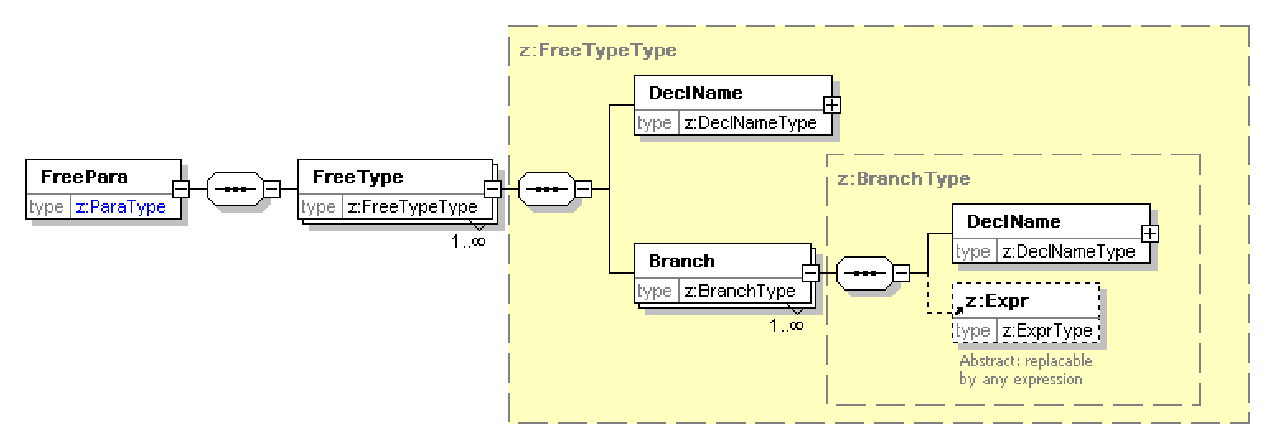
\includegraphics[width=\textwidth]{freepara.eps}
  \caption{XML structure for Free Type paragraphs}
  \label{fig:freepara}
\end{figure}


\subsubsection{Conjecture Paragraphs}

\Zeta\ does not support conjecture paragraphs.

In \CADiZ, conjectures are represented as particular cases of
a more general syntax for sequents.
Sequents allow for zero-or-more generic parameters,
zero-or-more levels of nested \AFont{DeclPart}s,
zero-or-more antecedent predicates,
zero-or-more consequent predicates,
and a name for the sequent.
This more general syntax assists humans doing proofs interactively,
but adds nothing semantically: any sequent can be rearranged
into an equivalent single-consequent form that conforms to the Z standard
(ignoring the sequent's name, which can be thought of as an annotation).
Other reasoning tools for Z may use different representations for sequents.
So it seems inappropriate to define an XML mark-up for anything
more complicated than a Standard Z (generic) conjecture.

The following table lists the components of a conjecture paragraph.

\begin{center}
\begin{tabular}{|l|l|}
\hline
{\bf Standard Z} & {\bf XML}\\
(Generic) conjecture \AParagraph & \AFont{Z:ConjPara}\\
\hline
\AFont{seq} \TNAME & \AFont{Z:DeclName*}\\
\APredicate & \AFont{Z:Pred}\\
\ASignature & \AFont{Z:ConjParaAnns?}\\
\hline
\end{tabular}
\end{center}

In XML, a conjecture paragraph is marked-up using
the \AFont{Z:ConjPara} element, as shown in Fig.~\ref{fig:conjpara}.
This representation suffices for both generic and non-generic
conjecture paragraphs: the sequence of generic parameters is empty in the
non-generic case. 

\begin{figure}[htbp]
  \centering
  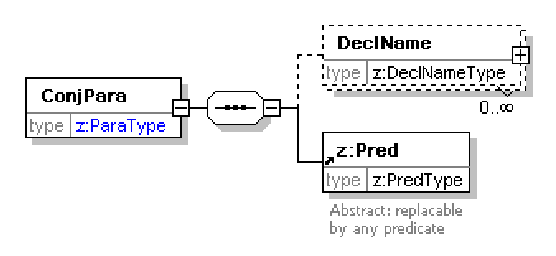
\includegraphics{conjpara.eps}
  \caption{XML structure for Conjecture paragraphs}
  \label{fig:conjpara}
\end{figure}


\subsubsection{Operator Template Paragraphs}

Standard Z has operator template paragraphs in its concrete syntax
but not in its annotated syntax,
because they affect how the specification is parsed
but have no further meaning themselves.
To be able to interchange them and resurrect their concrete syntax,
and the concrete syntax of the operators they define,
the XML mark-up must provide a representation of them.

Operator templates are one of the innovations of Standard Z
and were subject to some late changes,
so tools are unlikely to support operator templates exactly as in Standard Z
(excepting \CADiZ).
The concrete syntax allows explicit declaration of precedence and associativity
only for infix function and infix generic operators.
Other operators have implicit precedences and associativities,
which it is convenient to make explicit in the annotated syntax.

The following table lists the components of an operator template paragraph.

\begin{center}
\begin{tabular}{|l|l|l|l|}
\hline
{\bf Standard Z} & {\bf \CADiZ} & {\bf \Zeta} & {\bf XML}\\
Operator template \AParagraph & \AFont{fixdef} & \AFont{Fixity} & \AFont{Z:OptempPara}\\
\hline
\AFont{Category} & \AFont{cat} & \AFont{isGeneric} & \AFont{Z:Cat}\\
\CPrec & \AFont{nat} & \AFont{prio} & \AFont{Z:Numeral}\\
\CAssoc & \AFont{boole} & \AFont{?} & \AFont{Z:Assoc}\\
\AFont{Template} & \AFont{[nat,word]} & \AFont{Component[]} & \AFont{Z:Template}\\
\hline
\end{tabular}
\end{center}

In \CADiZ, a \AFont{Template} is represented as a list of pairs.
While this enforces alternation of operators and operands,
it may unfortunately appear to add an unwanted operand at the beginning
and/or an unwanted operator at the end,
for which distinguishable values are needed to avoid confusion.

In \Zeta, a \AFont{Template} is represented as a list of \AFont{Component}s.
Each \AFont{Component} is either a \AFont{Keyword}, \AFont{Operand} or
\AFont{OperandList}.
\Zeta\ appears to parse declarations of associativity,
but it does not appear to keep a representation of associativity
in its annotated syntax.
Its annotated syntax also appears not to distinguish
relation and function categories.

In XML, an operator template paragraph is marked-up using
the \AFont{Z:OptempPara} element, as shown in Fig.~\ref{fig:optemppara}.
In addition, each \AFont{Z:OptempPara} has three attributes:
\begin{description}
\item[\AFont{Cat}] (category) which can equal \AFont{Relation},
  \AFont{Function} or \AFont{Generic}.  
\item[\AFont{Assoc}] which can be \AFont{Left} or \AFont{Right}. 
\item[\AFont{Prec}] (precedence) which is an integer in the range $0 \upto
  9$.
\end{description}

\begin{figure}[htbp]
  \centering
  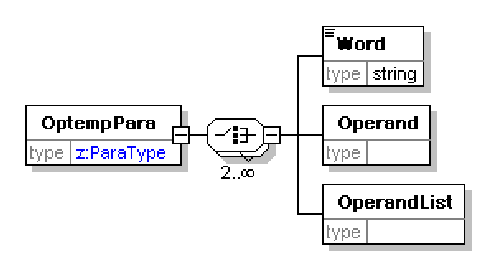
\includegraphics{optemppara.eps}
  \caption{XML structure for Operator Template paragraphs}
  \label{fig:optemppara}
\end{figure}


\subsubsection{Unparsed Paragraphs}

Our final kind of paragraph does not appear in \CADiZ, {\Zeta}
or the Z standard, because their annotated syntax representations
are used only \emph{after} an entire specification has been successfully
parsed.  However, since our XML format may be our source representation,
we need to be able to represent erroneous (unparsable) specifications as
well. 

\TODO{Expand this so that an entire section, and an entire specification
  can also be unparsed.  Or is putting ALL the unparsed stuff into one
  UnparsedPara a good enough solution?  (We can wrap a dummy Sect around it
  if the whole specification is unparsed).}

\begin{figure}[htbp]
  \centering
  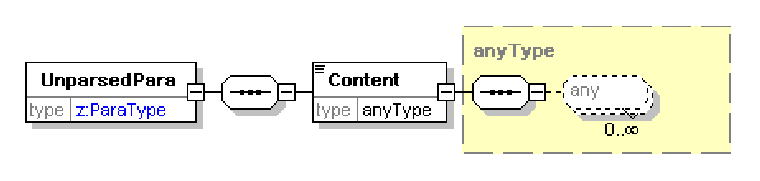
\includegraphics[width=\textwidth]{unparsedpara.eps}
  \caption{XML structure for Unparsed paragraphs}
  \label{fig:unparsed}
\end{figure}


\subsection{Predicates, Expressions and Types}

We shall not go into details about the structure of predicates and
expressions etc., but will discuss some specific features and give
a few short XML examples.

\TODO{Write a longer version of this paper which includes Ian's
  comparison of predicate and expression structures and rationale
  for their XML format.}

\TODO{Convert predicates to the `subtyping' style, like expressions?}

\TODO{Talk about ApplExpr and MemPred with their Fix attribute, RefExpr
  with its Square/Mixfix attribute, }

\TODO{Give small examples...}


\paragraph{The Challenge of Nested Identical Names}

In Z it is quite common to have several levels of declarations nested 
inside one another.  If two levels declare the same name $x$, then
expressions inside the inner scope cannot normally refer to the outer $x$.
However, there are situations where the instantiation of generic
operators during type checking must introduce references to the outer $x$.
This creates a problem, because naively introducing $x$ would cause it
to bind to the inner $x$ rather than the outer.

\TODO{Ian, can you remember the example that we worked out at ZB2002?}

None of the previous DTD or XML Schema proposals solve this problem.
To allow exact resurrection of concrete syntax, we do \emph{not} want to
rename the bound variables.  Instead, we use the ID and IDREF
crossreference features of XML to allow a variable reference to point to
a specific variable declaration (which may not be the nearest nested
name).  Since soundness relies on following these references correctly,
every Z tool must be capable of following them, and pretty printers must
display the output unambiguously (either by renaming one of the bound
variables, or by making the generic instantiations implicit again to hide
the problem reference).  

%% NOTE: The following idea was dropped, for several reasons.
%%    1. declaration becomes unparsed, while references to it stay parsed.
%%    2. In (\forall S @ x=3) the x will presumably point to the S, 
%%       but this does not uniquely determine the text of the name x.
%%
% Note that in variable references that contain an ID
% value, the actual name of the variable is redundant, since it can be
% obtained from the declaration.  For this reason, we decided to simplify
% \AFont{RefExpr} so that it always contains an ID attribute, rather than
% the word and decorations of the name.  That is, rather than writing
% \begin{verbatim}
%     <RefExpr><RefName><Word>name</Word><InStroke></RefName></RefExpr>
% \end{verbatim}
% to refer to the variable $name?$, we write just
% \begin{verbatim}
%     <RefExpr Decl="name?.3"></RefExpr>,  or
%     <RefExpr Decl="name?.3"/>,
% \end{verbatim}
% where the declaration of $name?$ contains the attribute
% \verb!Id="name?.3"!.  Note that human readability can be retained
% by using the variable name as a prefix of the ID label, as illustrated here.

% \begin{figure}[htbp]
%   \centering
%   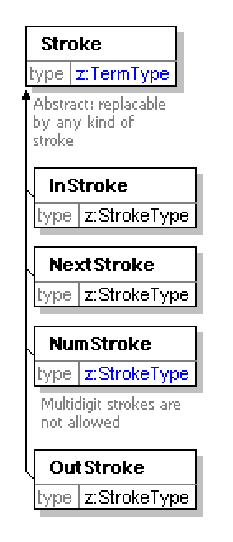
\includegraphics{stroke.eps}
%   \caption{XML structure for decorations (strokes) on names}
%   \label{fig:stroke}
% \end{figure}



\section{Support for Z Special Symbols}

% Adapted from http://nt-appn.comp.nus.edu.sg/fm/zml
Z/Object-Z languages use a rich set of mathematical symbols.  These
can be presented directly in Unicode within XML files (e.g., \verb!&#x2208!
is the membership symbol, $\mem$), but it is sometimes desirable to make
the XML files more human readable.  To support this, we have written a DTD
that uses entity declarations to give \LaTeX-compatible symbolic names to
all the Z operators (this is not possible in XML Schema, because it does
not support entity declarations).  Part of this DTD is:

\begin{small}
\begin{verbatim} 
<?xml version="1.0" encoding="UTF-8"?>
<!ENTITY emptyset "&#x2205;">
<!ENTITY mem "&#x2208;">
<!ENTITY pset "&#x2119;">
<!ENTITY fset "F">
<!ENTITY psetone "&#x2119;&#x2081;">
<!ENTITY fsetone "F&#x2081;">
\end{verbatim}
\end{small}


 
\section{Conclusions}

We have defined an XML markup format for standard Z, based on
combining the best features from the standard and several existing 
tools.  The XML schema has been validated, and several small examples
have been validated against the schema.  We are now seeking feedback 
and comments on the design.

The comparison has been worthwhile,
as can be seen by considering the main influences on the XML structure.
Specification's representation is influenced mainly by the form of XML.
Section's representation is influenced mainly by \Zeta.
Paragraph's representation is influenced mainly by Standard Z,
with the commonality between generics and non-generics taken from
both \CADiZ\ and \Zeta,
and the template representation in operator templates taken from \Zeta.
Predicate's representation is influenced mainly by \CADiZ\ and \Zeta,
which use remarkably similar representations.
Expression's representation falls between those of \CADiZ\ and \Zeta.
Schema text and name's representations are influenced mainly by \Zeta.

Next we plan to derive a set of open-source Java classes from this XML
schema, preferably by using XSLT to transform the schema into Java source.
These Java classes will support the visitor design
pattern~\cite{Patterns???}, so that functionality such as type checkers,
transformation tools, simplifiers and pretty printers can easily be written
as add-on packages.  This will dramatically reduce the usual initial
barriers of creating new Z tools (parsing, type-checking etc.) and make it
easier for student projects and other researchers to experiment with
building new Z tools.

Another important step is for existing Z tools to support this
XML format, by adding import and export functions that read and write it.
{\CADiZ} already exports an XML format that is close to this one.

Maybe copy some conclusions from http://nt-appn.comp.nus.edu.sg/fm/zml/ !

\bibliographystyle{plain}
\bibliography{cmp}
\end{document}
